\section{Reconstruction of Particle Collision Events in the ATLAS Detector}%
\label{sec:object_reco_at_atlas}

\subsection{Tracking, Vertexing, Topoclustering}
\subsection{Electrons}
\subsection{Muons}
\subsection{Jets and $b$-tagging}

\subsection{Hadronic Tau Lepton Decays}

\begin{figure}[htb]
  \begin{subfigure}[b]{0.47\textwidth}
    \centering

    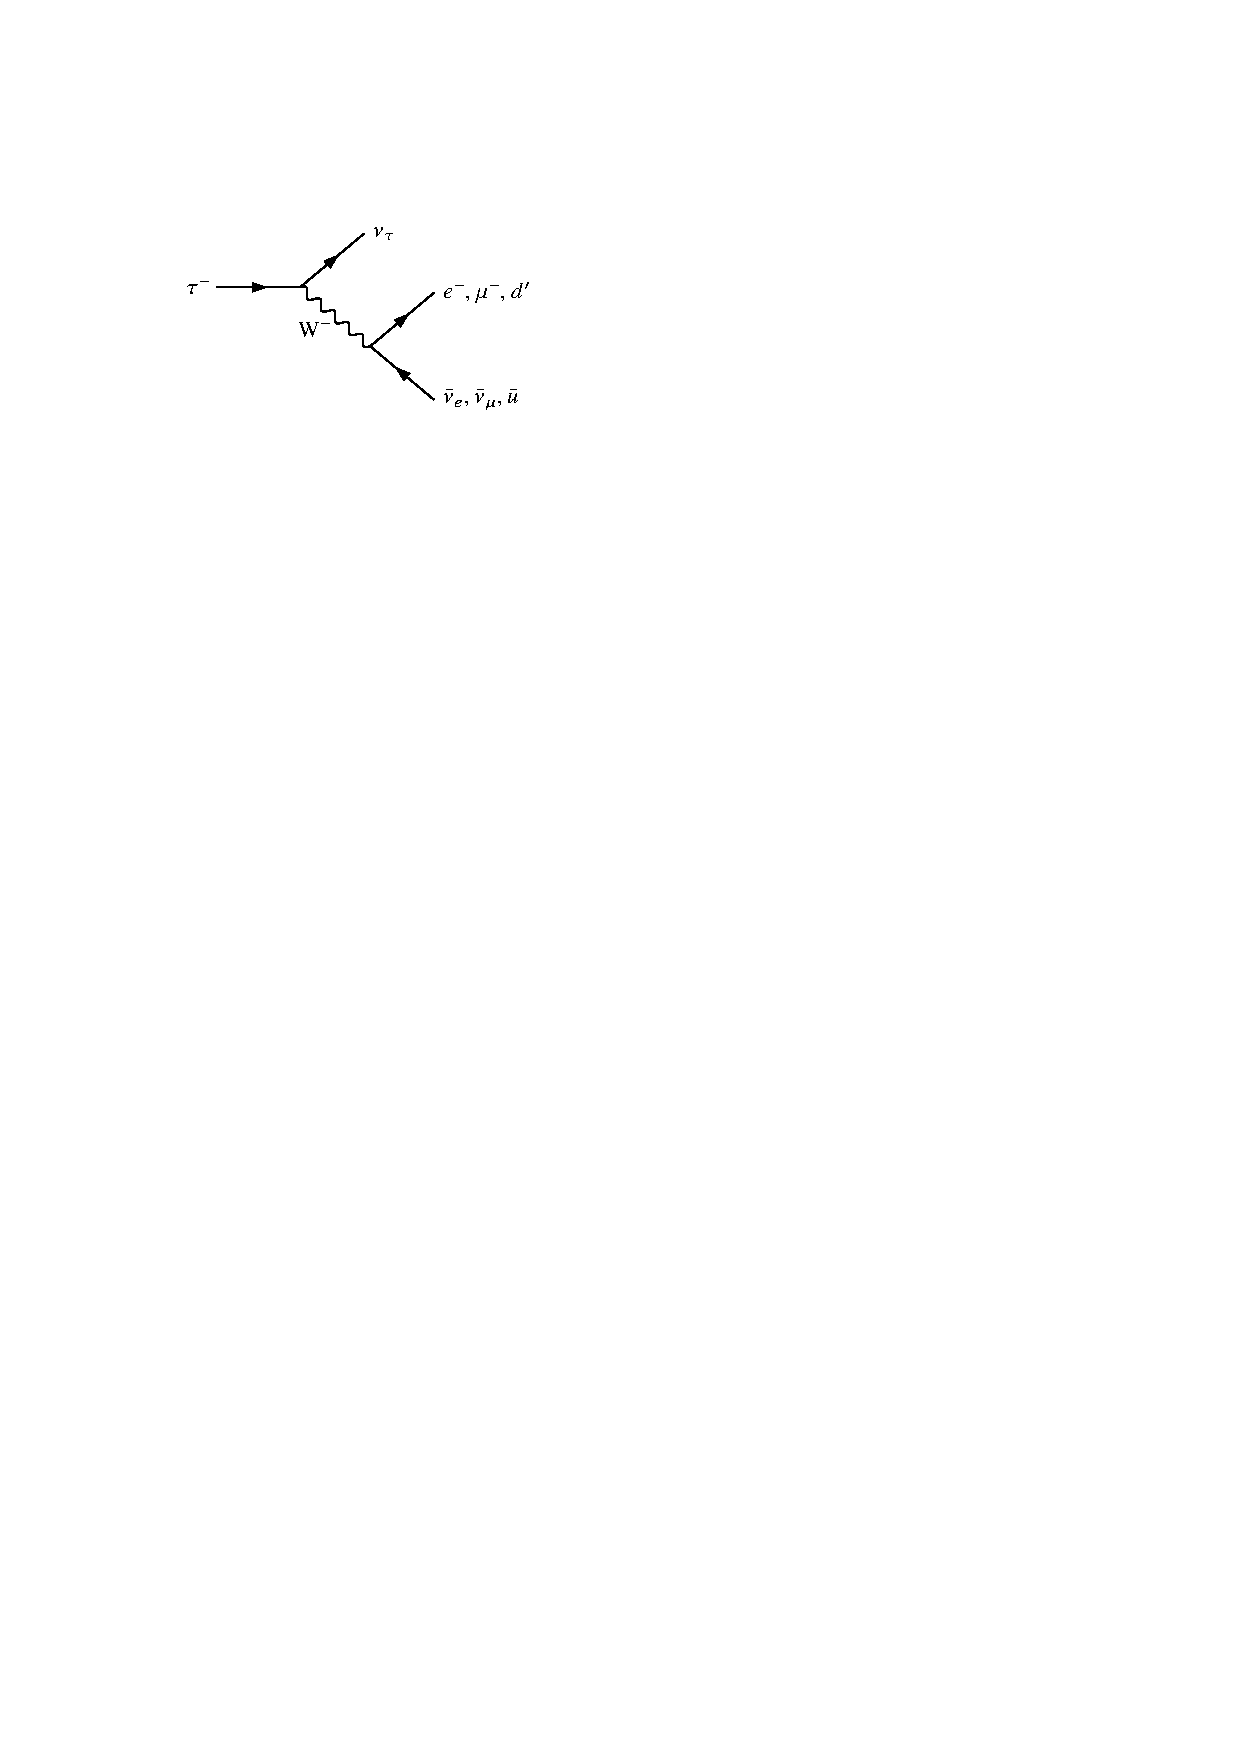
\includegraphics{figs/tauid/tau_decay_feynman}

    \vspace*{3em}
    \subcaption{a}%
    \label{fig:tau_feynman}
  \end{subfigure}\hfill
  \begin{subfigure}[b]{0.47\textwidth}
    \centering

    \begin{overpic}[scale=0.9]{figs/tauid/tau_branching_pie_chart}
      \put (31, 83) {$\pi^- \nu_\tau$}
      \put (-5.5, 45) {$\pi^- \pi^0 \nu_\tau$}
      \put (16, 7) {$\pi^- 2 \pi^0 \nu_\tau$}
      \put (40.5, 2) {$2 \pi^- \pi^+ \nu_\tau$}
      \put (65, 6.5) {$2 \pi^- \pi^+ \pi^0 \nu_\tau$}
      \put (76.5, 15.5) {other}
      \put (70, 77.5) {$e^- \bar{\nu}_e \nu_\tau$}
      \put (88.5, 41.5) {$\mu^- \bar{\nu}_\mu \nu_\tau$}
    \end{overpic}

    \subcaption{}%
    \label{fig:tau_branching_ratios}
  \end{subfigure}
  \caption{Decay and branching ratios of the tau
    lepton. Charge-conjugate decay modes are omitted.}
\end{figure}


\subsubsection{Seed Jet}

Seeded with AntiKt 0.4 jets on TopoClusters at the LC scale.

\subsubsection{Tau Vertex Association}

TJVA

\subsubsection{Track Association}

\cite{duschinger}

\todo[inline]{Make sure to point out the difference between ``tau
  tracks'' and all other tracks.}

\subsubsection{Energy Calibration}

MVA TES

\subsubsection{Electron Veto}
\subsubsection{Tau Identification}

\subsection{Missing Transverse Energy}

%%% Local Variables:
%%% mode: latex
%%% TeX-master: "../../phd_thesis"
%%% End:
